\documentclass[../main.tex]{subfiles}

\begin{document}

\section{Method}
\subsection{Data sets}
\subsubsection{Fashion-MNIST}
The fashion-MNIST is a dataset of Zalando's article images -- consisting of a training set of 60,000 examples and a test set of 10,000 examples \cite{xiao2017/online}. A sample of the dataset can be seen i \cref{fig:ex_fashion_MNIST}. Each article image is a \ensuremath{28\times28} grayscale image, associated with a label from 10 classes. The class labels can be seen in \cref{tab:labels}. The items are distributed evenly, 6000 of each in the training set and 1000 in the test set. As the fashion-MNIST shares the same image size and structure of training and testing splits, it can serve as a direct drop-in replacement for the original MNIST dataset for benchmarking machine learning algorithms. 

\begin{figure}[!htb]
    \centering
    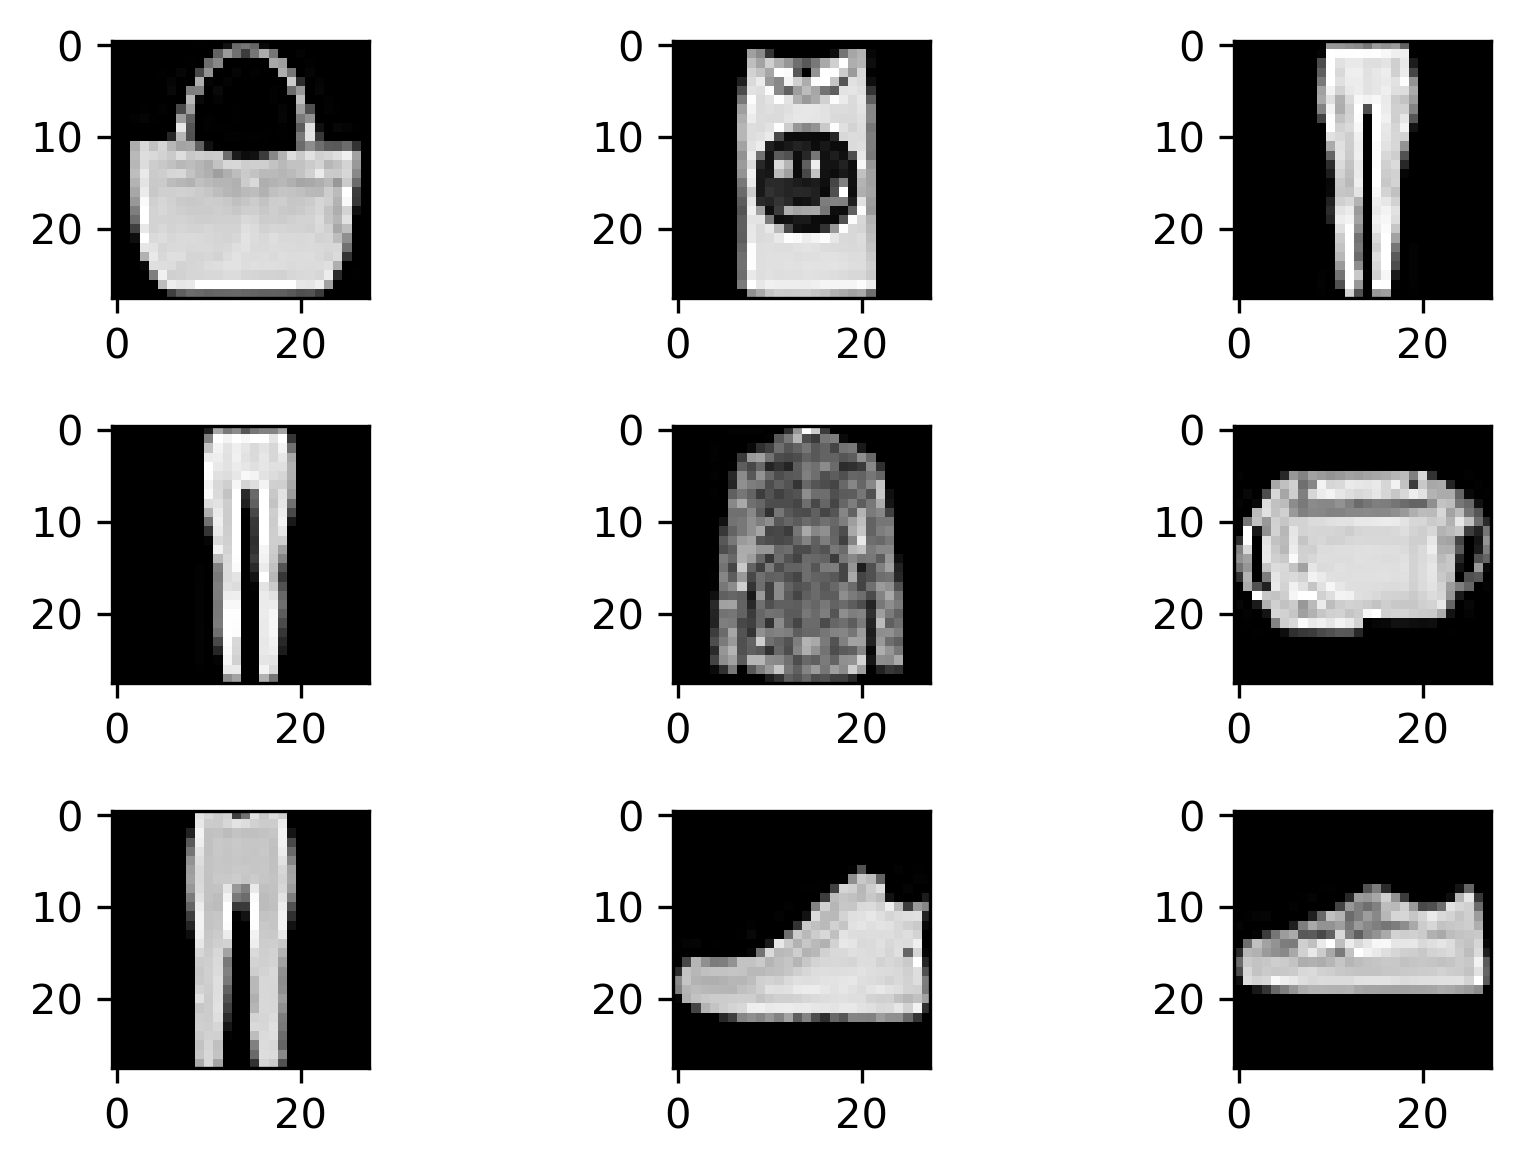
\includegraphics[width=0.8\textwidth]{doc/fig/example_fashion_mnist.png}
    \caption{A sample of the fashion-MNIST dataset.}
    \label{fig:ex_fashion_MNIST}
\end{figure}

\begin{table}[htb]
    \centering
    \caption{Class names in the fashion-MNIST dataset. }
    \begin{tabular}{c c}
    \toprule
    Label    & Description  \\
    \midrule
    0 & T-shirt/top \\
    1 & Trouser \\
    2 & Pullover \\
    3 & Dress \\
    4 & Coat \\
    5 & Sandal \\
    6 & Shirt \\
    7 & Sneaker \\
    8 & Bag \\
    9 & Ankle boot \\
    \bottomrule
    \end{tabular}
    \label{tab:labels}
\end{table}

\subsubsection{Facemask detection dataset}
The facemask dataset is a dataset consisting of approximately 4000 RGB images of sizes \ensuremath{1024\times1024}. The dataset consists of pictures of people with and without face masks. The images is split into two folders, a train- and a testset. The dataset can be found at kaggle\cite{facemask_dataset}. For easier handling of the images, the images were preprocessed and saved as arrays to make it easier to load when applying the models. The prehandling includes reshaping the images into sizes of \ensuremath{224\times224} pixels. The masks on the images were edited on by computer tools. Some of the photos can be seen in figure \ref{fig:ex_facemask_set}

\begin{figure}[H]
    \centering
    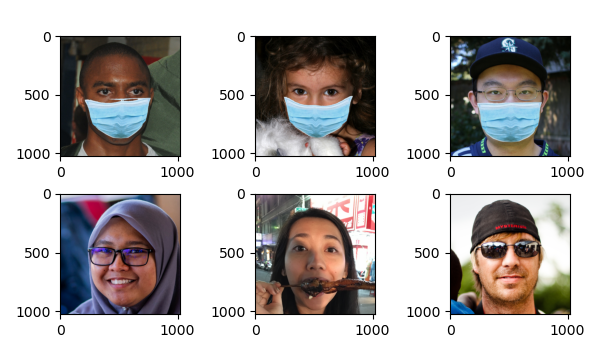
\includegraphics[width=0.8\textwidth]{doc/assets/face_mask_samples.png}
    \caption{A sample of the facemask detection dataset. The predicted value 1=mask, while the predicted value 0=no mask.}
    \label{fig:ex_facemask_set}
\end{figure}

\subsection{Logistic regression}
The implementation of the logistic regression is implemented pretty straight forward. From project 2 \cite{project2}, it was shown that scikit learn had the ability to provide predictions using logistic regression much faster, and a bit more accurate than a self written SGD algorithm. The logistic regression in this article therefore revolves around scikit learn's logistic regression library. Beside using scikit learn's machine learning library, scikit learn's image processing library which is as the name says, an image processing library. This well known library is quite useful when dealing with images, and was implemented when processing the images from the facemask dataset.

The facemask implementation is done by resizing the images into sizes of 224x224 to reduce the computer effort. Then the images is scaled by dividing the pixels by the maximum pixel value, and sorted into arrays. Then removing the present colours by transforming the images into grayscale. This way there is only one colour channel to work with, instead of the original three. The mnist dataset doesn't need as much prework as the facemask dataset except scaling the data.

After the data is ready, the pixel values are sent into the logistic regression function and trained. After the training is done, the fitting and predicting is ready to be set in motion. The predicted response vector for the datasets is retured, which then can be used to calculate the accuracy.


\end{document}